\section{Combinatorial Elastica}

\begin{frame}
\begin{center}
\huge
A combinatorial model for elastica
\end{center}
\end{frame}

\begin{frame}
	{Combinatorial Elastica}	
	{Digital elastica}
%	
		\begin{definition}[Digital elastica energy]
		Let $\hat{s}$ and $\hat{\kappa}$ multigrid convergent estimators of local length and curvature. The digital elastica energy of a digital shape $S \subset \Omega \subset \mathbb{Z}^2$ is defined as
%		
		\begin{align*}
			\hat{E}(S) = \sum_{e \in \partial_h(S)}{\hat{s}(e) \Big(\: \alpha + \beta \hat{\kappa}^2(e) \: \Big). }
		\end{align*}
	\end{definition}
%	
	\begin{itemize}
		\item<2->{\emph{Local search}: set a local neighborhood $\mathcal{N}(S)$ of $S$ and pick the shape $X^{\star} \in \mathcal{N}(S)$ among those of minimum digital elastica value.}
	\end{itemize}
\end{frame}

\begin{frame}
	{Combinatorial Elastica}	
	{Local search algorithm}

\begin{algorithm}[H]
 \SetKwData{It}{i}
 \SetKwData{MIt}{maxIt}
 \SetKwData{Tol}{tolerance}
 \SetKwData{Delta}{delta}
 \SetKwData{Best}{best} 
 \SetKwInOut{Input}{input}\SetKwInOut{Output}{output}
 
 \Input{A digital set $S$; coefficient $\alpha, \beta$; the maximum number of iterations \MIt; and a stop condition \Tol}
 \BlankLine
 \Delta $\longleftarrow$ \Tol+1\;
 $i \longleftarrow 0$\;
 $S^{(0)} \longleftarrow S$\;
 $X^\star \longleftarrow S$\;
 \While{ \color{black} \It $<$ \MIt \bf{and} \Delta $>$ \Tol  }{
  	\For{$\color{black} X \in \mathcal{N}(S^{(i)}) $}
	{
		\If{\color{black} $\hat{E}(X)$ $<$ $\hat{E}(X^\star)$ }
		{
			$X^\star \longleftarrow X$
		}
	}
	\It $\longleftarrow$ \It $+1$\;
	$S^{(i)} \longleftarrow X^\star$\;
	\Delta $\longleftarrow$ $\hat{E}(S^{(i-1)}) - \hat{E}(S^{(i)})$\;	
 }
\end{algorithm}
\end{frame}

\begin{frame}
	{Combinatorial Elastica}	
	{Neighborhood of shapes}
	
\begin{minipage}{0.49\textwidth}
\center
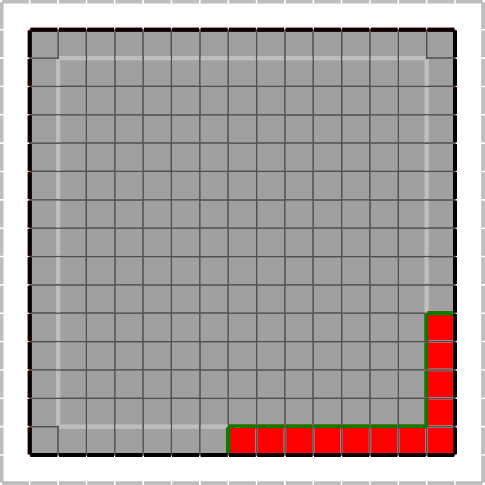
\includegraphics[scale=0.25]{figures/combinatorial-elastica/main-inner.png}	
\end{minipage}
\begin{minipage}{0.49\textwidth}
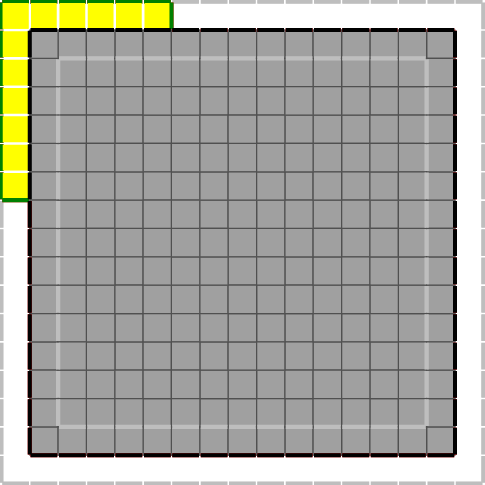
\includegraphics[scale=0.25]{figures/combinatorial-elastica/main-outer.png}	
\end{minipage}	
\end{frame}

\begin{frame}
	{Combinatorial Elastica}	
	{Shape evolution}

\begin{center}
$\alpha=0.01, \beta=1$
\end{center}
\begin{minipage}{0.49\textwidth}
\center
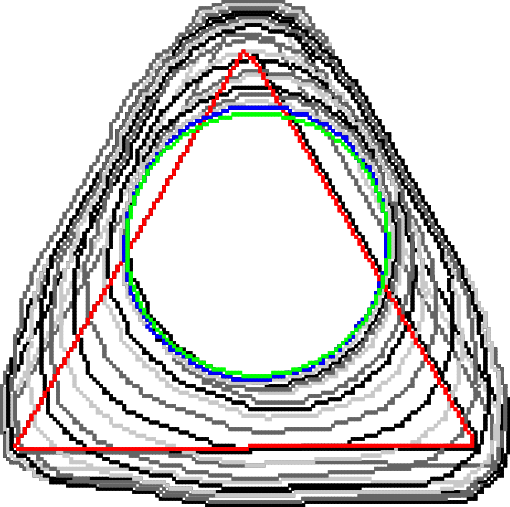
\includegraphics[scale=0.15]{figures/combinatorial-elastica/flow/ii/elastica/len_pen_0.01000/jonctions_1/curve_segs_4/best/gs_0.25000/triangle.png}\\[1em]
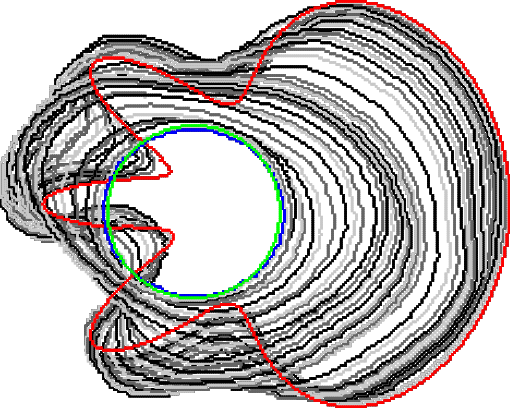
\includegraphics[scale=0.18]{figures/combinatorial-elastica/flow/ii/elastica/len_pen_0.01000/jonctions_1/curve_segs_4/best/gs_0.25000/flower.png}
\end{minipage}	
\begin{minipage}{0.49\textwidth}
\center
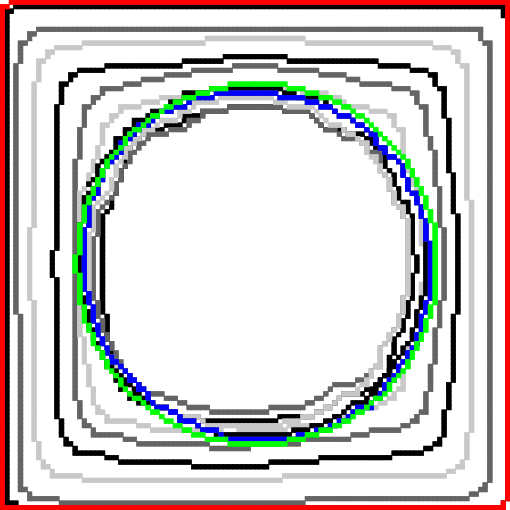
\includegraphics[scale=0.15]{figures/combinatorial-elastica/flow/ii/elastica/len_pen_0.01000/jonctions_1/curve_segs_4/best/gs_0.25000/square.png}\\[1em]
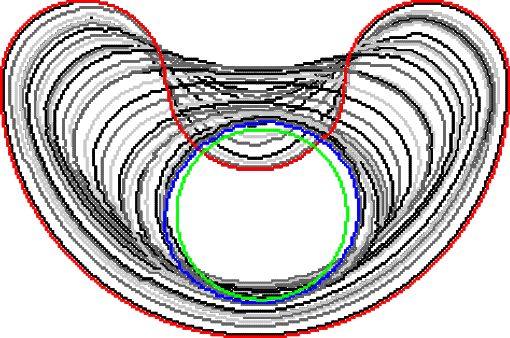
\includegraphics[scale=0.18]{figures/combinatorial-elastica/flow/ii/elastica/len_pen_0.01000/jonctions_1/curve_segs_4/best/gs_0.25000/bean.png}
\end{minipage}

\end{frame}

\begin{frame}
	{Combinatorial Elastica}	
	{Energy evolution}

\begin{minipage}{0.49\textwidth}
\center
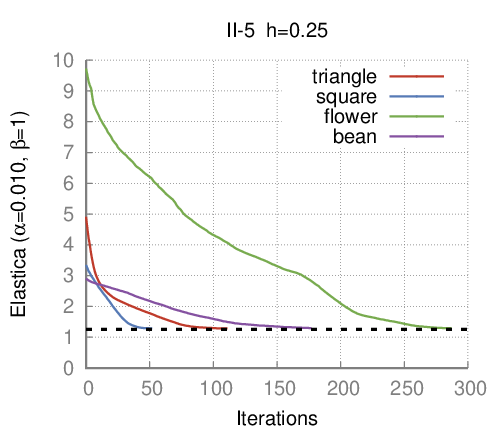
\includegraphics[scale=0.3]{figures/combinatorial-elastica/flow/ii/elastica/len_pen_0.01000/jonctions_1/curve_segs_4/best/gs_0.25000/summary-ii5.png}
\end{minipage}
\begin{minipage}{0.49\textwidth}
\begin{align*}
	\min E(X) &= \int_{\partial X}{ \alpha + \beta \kappa^2 ds}\\
	 &= 4\pi \beta \frac{1}{r} = 4\pi \beta \left(\frac{\alpha}{\beta}\right)^{1/2}
\end{align*}
, where $\frac{\partial }{\partial r} 2\pi(\alpha r + \frac{\beta}{r}) = 0$\\ 

%
For $\alpha=0.01,\; \beta=1$
%
\begin{align*}
	\min E(X) \approx 1.2566
\end{align*}
\end{minipage}
	
\end{frame}

\begin{frame}
	{Combinatorial Elastica}
	{Radius and grid resolution}
	
\begin{minipage}{0.49\textwidth}
\center
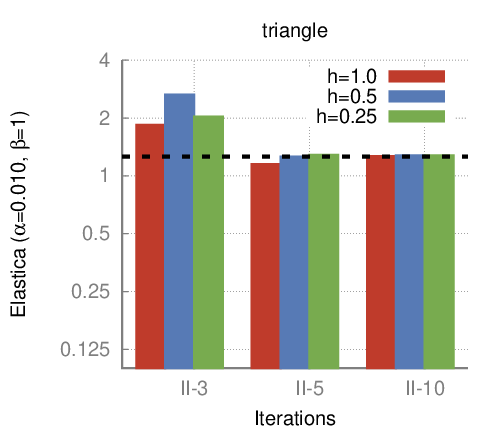
\includegraphics[scale=0.25]{figures/combinatorial-elastica/flow/ii/elastica/len_pen_0.01000/jonctions_1/curve_segs_4/best/gs_0.25000/triangle-bars.png}\\[0.6em]
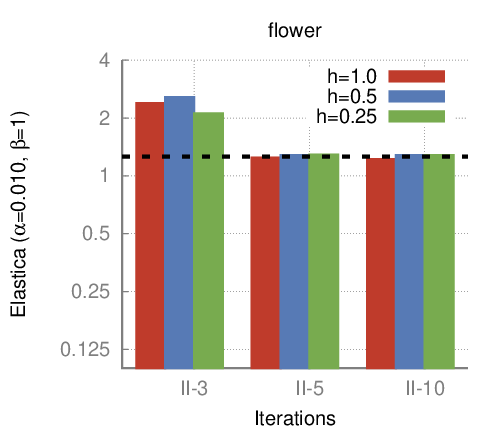
\includegraphics[scale=0.25]{figures/combinatorial-elastica/flow/ii/elastica/len_pen_0.01000/jonctions_1/curve_segs_4/best/gs_0.25000/flower-bars.png}
\end{minipage}	
\begin{minipage}{0.49\textwidth}
\center
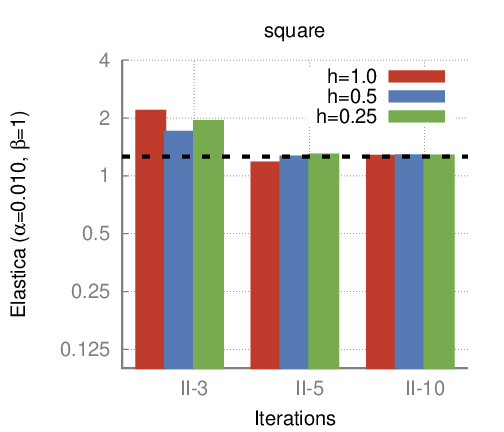
\includegraphics[scale=0.25]{figures/combinatorial-elastica/flow/ii/elastica/len_pen_0.01000/jonctions_1/curve_segs_4/best/gs_0.25000/square-bars.png}\\[0.6em]
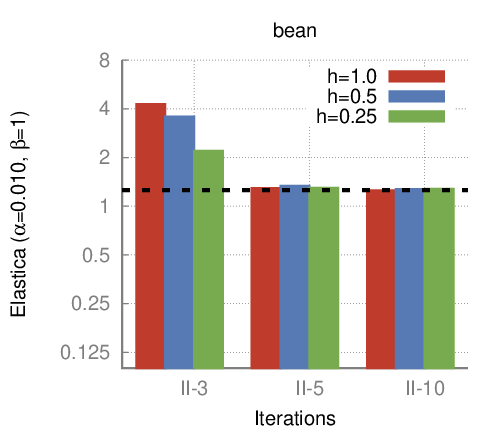
\includegraphics[scale=0.25]{figures/combinatorial-elastica/flow/ii/elastica/len_pen_0.01000/jonctions_1/curve_segs_4/best/gs_0.25000/bean-bars.png}
\end{minipage}
\end{frame}

\begin{frame}
	{Combinatorial Elastica}
	{Other experiments}
	
\begin{minipage}{0.49\textwidth}
\center
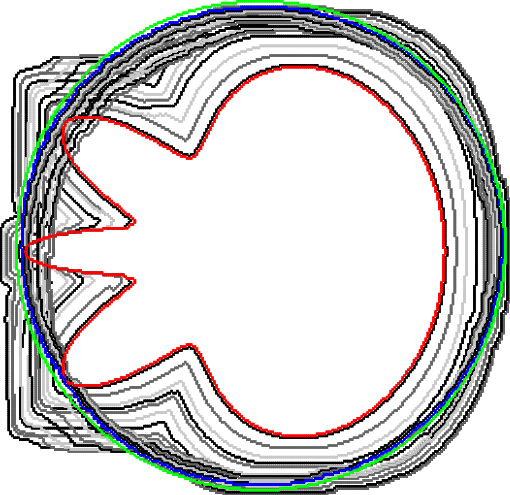
\includegraphics[scale=0.25]{figures/combinatorial-elastica/other-experiments/ii/elastica/len_pen_0.001000/jonctions_1/curve_segs_4/best/gs_0.25000/flower.png}
\end{minipage}
\begin{minipage}{0.49\textwidth}
\center
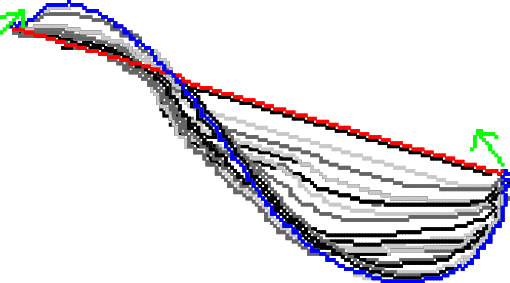
\includegraphics[scale=0.25]{figures/combinatorial-elastica/other-experiments/ii/elastica/len_pen_0.001000/jonctions_1/curve_segs_4/best/gs_0.25000/curve.png}
\end{minipage}
\end{frame}

\begin{frame}
{Combinatorial Elastica}
{Running time}
\begin{center}
\captionsetup{type=table}
\scriptsize
\begin{tabular}{|l|c|c|c|c|c|c|}
\hline
& \multicolumn{2}{c|}{$h=1.0$} & \multicolumn{2}{c|}{$h=0.5$} & \multicolumn{2}{c|}{$h=0.25$}\\
\hline
& Pixels & Time & Pixels & Time & Pixels & Time\\
\hline
Triangle & 521 & 2s (0.07s/it)  & 2080 & 43s (0.81s/it) & 8315 & 532s(4.8s/it)\\
Square & 841 & 0.9s (0.09s/it) & 3249 & 8s (0.3s/it) & 12769 & 102s (2s/it)\\
Flower & 1641 & 13s (0.24s/it) & 6577 & 209s (1.68s/it) & 26321 & 3534s (12.3s/it)\\
Bean  & 1574 & 7s (0.16s/it) & 6278 & 88s (1.08s/it) & 25130 & 1131s (6.4s/it)\\
Ellipse  & 626 & 1s (0.14s/it) & 2506 & 16s (0.44s/it) & 10038 & 286s (3.1s/it)\\
\hline
\end{tabular}
\caption{\textbf{Running time of LocalSearch.} The running times for the free elastica problem are displayed. Notice that even having a similar number of pixels, the square (bean) shape evolves much faster than the triangle (flower).}
\end{center}
\end{frame}

\begin{frame}
{Combinatorial Elastica}
{Conclusion}

\begin{itemize}
\item{Multigrid convergent estimators are suitable for elastica minimization}\pause
\item{A simple neighborhood is sufficient to escape bad local minima. Some solutions very close to global optimum.}\pause
\item{Too slow. It cannot be used in practice.}
\end{itemize}
\end{frame}